\chapter{Funciones}
\label{funcchap}

En el contexto de la programación, una {\bf función}
es usualmente una secuencia de sentencias con nombre
que realizan una computación. En Perl, las funciones
son usualmente llamadas {\bf subrutinas} y los dos términos
(por ahora) pueden considerarse  más o menos equivalente. Cuando defines
una función, especificas el nombre y la secuencia de sentencias.
Después, cuando quieras realizar la computación, puedes 
``invocar`` la función por el nombre y esto ejecutará la secuencia
de sentencias dentro de la definición de la función.
\index{function}

Perl viene como muchas funciones integradas que son muy útiles.
Ya has visto algunas de ellas: por ejemplo, {\tt say} es una función 
integrada, y veremos más en el curso de este libro. Y si Perl no tiene
una función que hace lo que deseas hacer, tu puedes construirla. Esto
te enseña lo básico de las funciones y cómo construir una.

\section{Llamadas de Funciones}
\label{functionchap}
\index{function!call}

Ya hemos visto algunos ejemplos de {\bf llamadas de funciones}:

\begin{verbatim}
> say 42;
42
\end{verbatim}
%
El nombre de la función es {\tt say}. La expresión que sigue el
nombre de la función se llama el {\bf argumento} de la función.
La función {\tt say} causa que el argumento se ha mostrado en 
la pantalla. Si necesitas pasar varios argumentos a la función, 
solo separa los argumentos con comas:

\begin{verbatim}
> say "La respuesta a la pregunta absoluta es ", 42;
La respuesta a la pregunta absoluta es 42
\end{verbatim}
%

Muchos lenguajes de programación requieren que los argumentos de
la función se encuentren dentro de paréntesis. Esto no es requerido
(y usualmente no recomendado) en Perl~6 para la mayoría de 
las funciones integradas (excepto cuando se necesita para 
precedencia), pero si usas paréntesis, deberías evitar insertar 
espacios entre el nombre de la función y el paréntesis izquierdo,
Por ejemplo, la función {\tt round} usualmente toma dos argumentos:
el valor a ser redondeado y la unidad o escala.
Puedes invocarla en cualquiera de las siguientes formas:

\begin{verbatim}
> round 42.45, 1;
42
> round 42.45, .1;
42.5
> round(42.45, .1);      # Pero no: round (42.45, .1);
42.5
> round( 42.45, .1);     # Espacio *después* del paréntesis izq. es OK 
42.5
\end{verbatim}
\index{parentheses!argument in}

Los programadores de Perl con experiencia prefieren omitir los 
paréntesis cuando ellos pueden. Esto hace posible encadenar varias 
funciones con una sintaxis más limpia. Considera por ejemplo
la diferencia entre estas dos llamadas:

\begin{verbatim}
> say round 42.45, 1;
42
> say(round(42.45, 1));
42
\end{verbatim}

La segunda sentencia dice explícitamente lo que está pasando,
pero la acumulación de paréntesis actualmente no hace las cosas
muy claras. Por el contrario, la primera sentencia puede ser
considerada como una línea de tuberías que se puede leer de derecha 
a izquierda: la última función a la derecha, {\tt round}, toma dos
argumentos, {\tt 42.45, 1}, y el valor producido por {\tt round}
es pasado como un argumento a {\tt say}.

Es muy común decir que una función ``toma`` uno o varios
argumentos y ``devuelve`` un resultado. El resultado es también
llamado el {\bf valor de retorno}.
\index{argument}
\index{return!value}

Perl provee varias funciones que convierten valores de un
tipo a otro. Cuando se invocan con un solo argumento,
la función {\tt round} toma cualquier valor y lo convierte
en un número entero, o por el contrario se queja:
\index{conversion!type}
\index{type!conversion}
\index{round function}
\index{function!round}

\begin{verbatim}
> round 42.3;
42
> round "yes"
Cannot convert string to number: base-10 number must begin with valid 
digits or '.' in '<HERE>yes' (indicated by <HERE>)
  in block <unit> at <unknown file> line 1
\end{verbatim}

%
Nota que, en Perl~6, muchas funciones integradas pueden también
usar la sintaxis de la \emph{llamada de método} con la así 
llamada notación de punto. Las siguientes sentencias muestran el 
mismo resultado:
\index{invocation!method}
\index{method invocation}
\begin{verbatim}
> round 42.7;    # Sintaxis de la llamada de función
43
> 42.7.round;    # Sintaxis de la llamada de método
43
\end{verbatim}
%
La función {\tt round} puede redondear valores racionales
y valores coma flotante. Hay un método {\tt Int} que también
convierte valores numéricos no enteros en enteros, pero
no redondea; corta la parte fraccional:
\index{Int method}
\index{method!Int}

\begin{verbatim}
> round 42.7
43
> 42.7.Int
42
\end{verbatim}

Volveremos a los métodos en la siguiente sección.

La función integrada {\tt Rat} convierte números
enteros y cadenas de texto en números racionales (si es posible):
\index{Rat function}
\index{function!Rat}

\begin{verbatim}
> say 4.Rat;
4
> say 4.Rat.WHAT;
(Rat)
> say Rat(4).WHAT;
(Rat)
> say Rat(4).nude;
(4 1)
> say Rat('3.14159');
3.14159
> say Rat('3.14159').nude
(314159 100000)
\end{verbatim}
%
(Como podrás recordar de la Sección~\ref{values_and_types}, 
el método \verb'nude' muestra el \emph{nu}merador y  
\emph{de}nominador de un número racional.)

Finalmente, {\tt Str} convierte su argumento a una cadena de texto:
\index{Str function}
\index{function!Str}

\begin{verbatim}
> say 42.Str.WHAT
(Str)
> say Str(42).WHAT;
(Str)
\end{verbatim}

\index{coercion}
\index{type!coercion}
Nota que estas funciones de conversión de tipo no necesitan ser
invocadas explícitamente, dado que Perl intentará hacer lo correcto
en muchos de los casos. Por ejemplo, si tienes una cadena de texto
que se parece a un número entero, Perl \emph{coaccionará} la cadena 
de texto en un entero para ti si tratas de aplicarle una operación 
aritmética:

\begin{verbatim}
> say "21" * "2";
42
\end{verbatim}

Igualmente, los enteros serán coaccionados en cadenas de texto
si aplicas el operador de la concatenación de cadena de texto
sobre ellos:

\begin{verbatim}
> say 4 ~ 2;
42
> say (4 ~ 2).WHAT;
(Str)
\end{verbatim}

La coacción puede hasta pasar dos veces dentro de la misma expresión
si necesario:

\begin{verbatim}
> say (4 ~ 1) + 1;
42
> say ((4 ~ 1) + 1).WHAT;
(Int)
\end{verbatim}

\section{Funciones y Métodos}
\index{function}
\index{method}

Un método es similar a una función---toma argumentos y 
devuelve un valor---pero la sintaxis de llamada es
diferente. Con una función, especificas el nombre de la función
seguido de sus argumentos. Un método, por el contrario, usa 
la notación de punto: tu especificas el nombre del objecto
sobre el cual el método es invocado, seguido por un punto y
el nombre del método (y posiblemente argumentos adicionales).

% 
Una llamada de método es usualmente conocida como una 
{\bf invocación} \index{invocation}. Las diferencias más
profundas entre funciones y métodos se volverá aparente 
más adelante, cuando estudiemos la programación orientada
a objetos (en el Capítulo~\ref{objects}).
\index{invocation!method}
\index{method invocation}

Por el tiempo presente, podemos consider que la diferencia
es esencialmente un asunto de una sintaxis diferente de 
llamada cuando se usan las funciones integradas de Perl. La mayoría
de las funciones integradas en Perl aceptan la sintaxis de la llamada
de función y la sintaxis de la invocación de método. Por ejemplo,
las siguientes sentencias son equivalentes:

\begin{verbatim}
> say 42;              # sintaxis de la llamada de función
42
> 42.say;              # sintaxis de la invocación de método
42
\end{verbatim}
%

También puedes encadenar subrutinas con ambas formas
sintácticas:

\begin{verbatim}
> 42.WHAT.say;         # sintaxis de método
(Int)
> say WHAT 42;         # sintaxis de función
(Int)
> say 42.WHAT;         # sintaxis mixta
(Int)
\end{verbatim}
%

Depende de ti cuál de las formas prefieres usar, pero
usaremos ambas formas, aún solo sea para acostumbrarnos
a ambas.

\section{Funciones Matemáticas}
\index{math function}
\index{function!math}

Perl provee muchas de las funciones matemáticas familiares.

Para algunas funcionesno tan comunes, podría necesitar un
módulo especializado tal com \verb'Math::Matrix' o
\verb'Math::Trig'. Un {\bf módulo} es un archivo de texto 
que contiene una colección de funciones que están relacionadas.
\index{module}

Antes de que usemos las funciones en un módulo, tenemos que importarlo
la sentencia {\bf use}:

\begin{verbatim}
use Math::Trig;
\end{verbatim}
%
Esta sentencia importará un número de funciones que serás capaz de usar
como si tu las hubieses definido en el archivo de código principal,
por ejemplo \verb|grad2rad| convierte un valor angular desde grados
a radianes o \verb|rad2grad| que hace la conversión opuesta.

Para la mayoría de funciones matemáticas comunes, sin embargo, no necesitas
tener ningún módulo \verb|matemático|, dado que dichas funciones
ya están incluidas en núcleo del lenguaje:

\begin{verbatim}
> my $nivel-ruido = 5.5;
5.5
> my $nivel-señal = 125.6;
125.6
> my $decibelios = 10 * log10 $nivel-señal / $nivel-ruido;
13.5862694990693
\end{verbatim}
%
\index{log10 function}
\index{function!log10}
El primer ejemplo usa \verb"log10" (logaritmo común)
para computar la razón de señal y ruido en decibelios
(asumiendo que \verb|nivel-señal| y \verb|nivel-ruido| sean 
definidos en las propias unidades). Perl también provee una 
función {\tt log}, la cual, cuando recibe un argumento,
computa el logaritmo en base {\tt e} del argumento y,
cuando recibe dos argumentos, computa el logaritmo del primer
argumento en base del segundo argumento:

\begin{verbatim}
> say e;                 # e es predefinada como la constante de Euler
2.71828182845905
> my $val = e ** e;
15.1542622414793
> say log $val;          # logaritmo natural
2.71828182845905
> say log $val, e;       # logaritmo en base e o logaritmo natural
2.71828182845905
> say log 1024, 2;       # logaritmo binario o logaritmo en base 2
10
\end{verbatim}
%
\index{log function}
\index{function!log}

Perl también provee muchas de las funciones trigonométricas
comunes:

\begin{verbatim}
> my $radianes = 0.7;
0.7
> my $altura = sin $radianes;
0.644217687237691
\end{verbatim}

\index{sin function}
\index{radian}
\index{trigonometric function}
\index{function!trigonometric}
Este ejemplo encuentra el seno de \verb|$radianes|. El 
nombre de la variable es una pista a que el {\tt sin} y 
otras funciones trigonométricas ({\tt cos}, {\tt tan}, etc.) toman
argumentos en radianes. Para convertir de grados a radianes, puedes
usar la función \verb'deg2rad' del  módulo \verb|Math::Trig|, o
simplemente divide por 180 y multiplica por $\pi$:

\begin{verbatim}
> my $grados = 45;
45
> my $radianes = $grados / 180.0 * pi;    # pi, constante predefinida 
0.785398163397448
> say sin $radianes;       # debería ser la raíz cuadrada de 2 divida por 2
0.707106781186547
\end{verbatim}
%
La expresión {\tt pi} es una constante predefinida de una
aproximación de $\pi$, precisa alrededor de 14 dígitos:
\index{pi}

Si sabes trigonometría, puedes verificar el resultado anterior
al compararlo con la raíz cuadrada de 2 dividida por 2:
\index{sqrt function}
\index{function!sqrt}

\begin{verbatim}
> say sqrt(2) / 2;
0.707106781186548
\end{verbatim}
%

\section{Composición}
\index{composition}

Hasta ahora, hemos discutidos los elementos de un programa---variables,
expresiones, y sentencias---aisladamente, sin discutir sobre
cómo combinarlos.

Una de las características más útiles de los lenguajes de programación
es su habilidad de tomar pequeños componentes y {\bf componer} estos
componentes, i.e.,
combinarlos de tal manera que el resultado de uno es la entrada
de otro. Por ejemplo, el argumento de una función  puede ser cualquier
tipo de expresión, incluyendo operadores aritméticos:

\begin{verbatim}
> my $grados = 45;
45
> my $altura = sin($grados / 360.0 * 2 * pi);
0.707106781186547
\end{verbatim}
%
Aquí, hemos usados paréntesis para el argumento de la función
{\tt sin} para clarificar que todas las operaciones aritméticas
sean completadas antes que la función {\tt sin} sea actualmente
llamada, para que así use el resultado de estas operaciones 
como su argumento.

Puedes componer llamadas de funciones:

\begin{verbatim}
> my $x = 10;
10
>  $x = exp log($x+1)
11
\end{verbatim}
%
Casi en cualquier lado que puedes poner un valor, puedes poner
una expresión arbitraria, con una excepción: el lado izquierdo 
de la sentencia de asignación tiene que ser el nombre de una
variable, posiblemente con su declaración. Casi cualquier otra expresión
en el lado izquierdo es un error sintáctico \footnote{Veremos esta rara
excepción a esta regla más tarde}:


\begin{verbatim}
> my $horas = 1;
1
> my $minutos = 0;
0
> $minutos = $horas * 60;        # correcto 
60
> $horas * 60 = $minutos;        # incorrecto!!
Cannot modify an immutable Int
  in block <unit> at <unknown file> line 1
\end{verbatim}
%
\index{syntax error}


\section{Agregar Nuevas Funciones (o Subrutinas)}

\index{subroutine}
Hasta ahora, hemos solo usado las funciones que vienen con Perl,
pero también es posible agregar nuevas funciones. En Perl, las 
funciones definidas por el usuario son usualmente conocidas 
como subrutinas, pero podrías eligir cualquiera de las dos
palabras. 

Una {\bf definición de función} comienza con la palabra clave 
{\tt sub} (abreviación de subrutina) y especifica el nombre de una
nueva subrutina y la secuencia de sentencias que serán ejecutadas
cuando función es llamada.
\index{function}
\index{function!definition}
\index{definition!function}
\index{sub}

Este es un ejemplo de una subrutina que cita el famoso discurso
"I Have a Dream" de Martin Luther King en el Lincoln Memorial en
Washington (1963):

\begin{verbatim}
sub imprimir-discurso() {
    say "Let freedom ring from the prodigious hilltops of New Hampshire.";
    say "Let freedom ring from the mighty mountains of New York.";
}
\end{verbatim}
%
{\tt sub} es la palabra clave que indica que esto es una definición 
de subrutina. El nombre de la función es \verb|imprimir-discurso|.
Las reglas para los nombres de subrutinas son las mismas reglas 
para los nombres de variables: letras, números, y guiones bajos son
legales, al igual que un guión o un apóstrofo entre letras, pero
el primer carácter debe ser una letra o un guion bajo. No deberías
usar una palabra clave usada por el lenguaje (tales como {\tt if} 
o {\tt while}) como el nombre de una función (en algunos casos, podría
actualmente funcionar pero sería algo confuso, por lo menos 
para el lector humano).
\index{sub!keyword}
\index{keyword!sub}
\index{argument}

Los paréntesis vacíos después del nombre indican que esta función 
no toma ningún argumento. En tal caso los argumentos son opcionales,
pero son requeridos cuando los parámetros necesitan ser definidos para
la subrutina.
\index{parentheses!empty}
\index{header}
\index{body}

\index{indentation}
La primera línea de la definición de una subrutina es algunos
veces llamada la {\bf cabecera}; el resto es conocido como el
{\bf cuerpo} de la subrutina. El cuerpo tiene que ser un bloque de
código colocado entre llaves y puede contener una cantidad
indefinida de sentencias. Aunque no existe una regla que lo requiera,
es buena práctica (y muy recomendada) la indentación de las sentencias
en el cuerpo con varios espacios delanteros, debido a que facilita
descifrar visualmente donde el cuerpo de la función inicia y termina.
\index{curly bracket}
\index{curly brace}
\index{bracket!curly}

Ten presente que no puedes utilizar la sintaxis de invocación de método
con las subrutinas (tal como \verb|imprimir-discurso|) que escribas: 
debes llamarlas con la sintaxis de llamada de función.
\index{method!invocation}
\index{function!call}
\index{invocation!method}
\index{method invocation}

Las cadenas de texto en las sentencias de impresión están rodeadas
por comillas inglesas. En este caso específico, las comillas simples
se podrían haber usado para obtener el mismo resultado, pero
hay otros casos donde los dos tipos de comillas no harían lo mismo,
así que tendrás que elegir una de las dos dependiendo de las 
circunstancias.
\index{double quote}
\index{quote!double}
\index{single quote}
\index{quote!single}

Muchas personas usan las comillas inglesas en los casos
donde una comilla simple (la cual también es un apóstrofo)
aparece en una cadena de texto:
\index{apostrophe}
\begin{verbatim}
say "And so we've come here today to dramatize a shameful condition.";
\end{verbatim}
%
De igual manera, podrías utilizar comillas simples 
cuando las comillas inglesas aparecen en una cadena de texto:
\begin{verbatim}
say 'America has given the Negro people a bad check, 
     a check which has come back marked "insufficient funds."';
\end{verbatim}
%
Sin embargo, existe una diferencia más importante entre las 
comillas simples y las comillas inglesas: las comillas inglesas
permiten la interpolación de variables, lo cual no es posible
con el uso de comillas simples. La interpolación de variables
se refiere a que si el nombre de una variable aparece dentro
de una cadena de texto rodeada por comillas inglesas, dicho 
nombre será reemplazado por el valor de la variable; dentro una 
cadena de texto rodeada por comillas simples, el nombre de la 
variable aparecerá literalmente.
Por ejemplo:
%
\begin{verbatim}
my $var = 12;
say "La edad del niño es $var.";         # -> La edad del niño es 12.
say 'La edad de la niña es $var.';       # -> La edad de la niña es $var.
\end{verbatim}
\index{interpolation}
\index{variable!interpolation}
%
La edad de la niña no se muestra porque se quiera mantener un
secreto. En la primera cadena de texto, \verb|$var| es 
simplemente reemplazada dentro de la cadena por su valor, 12, porque
la cadena de texto está rodeada con comillas inglesas; en la segunda
cadena de texto, \verb|$var| no es reemplazada por su valor porque las 
comillas simples están supuestas a proveer un citado más literal. 
Existen otros tipos de citados que ofrecen un mayor control sobre la
manera en que las variables y los caracteres especiales son mostrados 
en la salida, pero las comillas simples y las comillas inglesas
son las más útiles.

La sintaxis para llamar una nueva subrutina es la misma usada
para llamar las funciones integradas:

\begin{verbatim}
> imprimir-discurso();
Let freedom ring from the prodigious hilltops of New Hampshire.
Let freedom ring from the mighty mountains of New York.
\end{verbatim}
%

No obstante, no puedes utilizar la sintaxis de invocación de método
con tales subrutinas. Más tarde veremos en este libro (ve
Capítulo~\ref{objects}) cómo crear métodos. Por el tiempo presente,
permaneceremos con la sintaxis de llamada de función.
\index{invocation!method}
\index{method invocation}

Una vez que has definido una subrutina, puedes usarla dentro
de otra subrutina. Por ejemplo, para repetir el fragmento anterior
del discurso de King, podríamos escribir una subrutina llamada 
\verb|repetir-discurso|:

\begin{verbatim}
sub repetir-discurso() {
    imprimir-discurso();
    imprimir-discurso();
}
\end{verbatim}
%
Y después llamar \verb|repetir-discurso|:

\begin{verbatim}
> repetir-discurso();
Let freedom ring from the prodigious hilltops of New Hampshire.
Let freedom ring from the mighty mountains of New York.
Let freedom ring from the prodigious hilltops of New Hampshire.
Let freedom ring from the mighty mountains of New York.
\end{verbatim}
%
No obstante, no es así como prosigue el discurso.


\section{Definiciones y Usos}
\index{function!definition}

Juntando los fragmentos de código de la sección anterior, el
programa entero luce así:

\begin{verbatim}
sub imprimir-discurso () {
    say "let freedom ring from the prodigious hilltops of New Hampshire.";
    say "Let freedom ring from the mighty mountains of New York.";
}
sub repetir-discurso () {
    imprimir-discurso();
    imprimir-discurso();
}
repetir-discurso();
\end{verbatim}
%
Este programa contiene dos definiciones de subrutinas: \verb|imprimir-discurso|
y \verb|repetir-discurso|. Las definiciones de funciones pueden ser ejecutadas
como otras sentencias, pero el efecto es crear la función. Las sentencias
dentro de la función no son ejecutadas hasta que la función es llamada, y
la definición de la función no genera ninguna salida.

No necesitas crear una subrutina antes de ejecutarla,
la definición de la función puede venir después de la llamada:

\begin{verbatim}
repetir-discurso;
sub repetir-discurso() {
    imprimir-discurso;
    imprimir-discurso;
}
sub imprimir-discurso() {
    # ...
}
\end{verbatim}


\section{Flujo de Ejecución}
\index{flow of execution}

Para asegura, por ejemplo, que una variable está definida (i.e. poblada)
antes de sus uso, necesitas saber el orden en el que las sentencias se
ejecutan. Dicho orden es conocido como el {\bf flujo de ejecución}.

La ejecución siempre con la primera sentencia del programa (bueno, {\bf casi}
siempre, pero digamos siempre por el tiempo presente). Las sentencias se
ejecutan una por una, de arriba hacia abajo.

Las definiciones de subrutinas no cambian el flujo de ejecución del 
programa, pero debes recordar que las sentencias dentro de una función
no son ejecutadas hasta que la función es llamada.

Una llamada de función es como un desvío en el flujo de ejecución. En vez
de continuar con la siguiente sentencia, el flujo salta al cuerpo de la función,
ejecuta las sentencias ahí dentro, y regresa para continuar donde se
quedó.

Esto suena simple hasta que recuerdas que una función puede llamar otra función.
Mientra se encuentra dentro de una función, el programa podría ejecutar las
sentencias en otra función. ¡Después, mientra se encuentra en dicha función,
el programa podría aún ejecutar otra función!

Afortunadamente, Perl es lo suficientemente bueno para rastrear dónde 
se encuentra, así que cada vez una función se completa, el programa continúa 
donde se quedó en el programa que lo llamó. Cuando llega al final del programa,
entonces termina.

En resumen, cuando leas un programa, no siempre quieras leerlo de 
arriba hacia abajo. Algunas hace más sentido si sigues el flujo de
ejecución.

\section{Parámetros y Argumentos}
\label{parameters}
\index{parameter}
\index{function!parameter}
\index{argument}
\index{function!argument}

Algunas de la funciones que hemos requieren argumentos. Por ejemplo,
cuando llamas a {\tt sin} tu le pasas un número como argumento. Algunas
funciones toman más de un argumento: por ejemplo, la función {\tt round}
que vimos al principio de este capítulo tomó dos, el número a ser redondeado
y la escala (aunque la función {\tt round} puede aceptar un solo 
argumento. En dicho caso, el valor de la escala por defecto es 1).
 
Dentro de la subrutina, los argumentos son asignados a variables llamadas 
{\bf parámetros}. Aquí está la definición de una subrutina que toma un 
solo argumento:
\index{parentheses!parameters in}

\begin{verbatim}
sub doble-impresión($valor) {
    say $valor;
    say $valor
}
\end{verbatim}
%
Esta subrutina asigna el argumento al parámetro llamado
\verb|$valor|. Otra manera común de interpretarlo es decir que
la subrutina ata el parámetro definido en su cabecera al argumento
con el cual es llamada. Cuando la subrutina anterior es llamada, 
imprimer el contenido del parámetro (cualquier cosa que sea) dos
veces.

Esta función funciona con cualquier argumento que pueda ser
imprimido:

\begin{verbatim}
> doble-impresión("Let freedom ring")
Let freedom ring
Let freedom ring
> doble-impresión(42)
42
42
> doble-impresión(pi)
3.14159265358979
3.14159265358979
\end{verbatim}
%
Las mismas reglas de composición que aplican a la funciones integradas 
también aplican a las funciones definidas por el programador, así que podemos
cualquier tipo de expresión como un argumento para \verb|doble-impresión|:
\index{composition}
\index{programmer-defined function}
\index{function!programmer defined}

\begin{verbatim}
> doble-impresión('Let freedom ring! ' x 2)
Let freedom ring! Let freedom ring! 
Let freedom ring! Let freedom ring! 
> doble-impresión(cos pi)
-1
-1
\end{verbatim}
%
El argumento es evaluado antes que la función sea llamada, 
así que en los ejemplos las expresiones \verb"'Let freedom ring! ' x 2" 
y {\tt cos pi} son evaluadas una sola vez.
\index{argument}

También puedes usar una variable como argumento:

\begin{verbatim}
> my $declaración = 'When in the Course of human events, ...'
> doble-impresión($declaración)
When in the Course of human events, ...
When in the Course of human events, ...
\end{verbatim}
%
El nombre de la variable que pasamos como un argumento (\verb|$declaración|)
no tiene nada que ver con el nombre del parámetro (\verb|$valor|). No
importa cual sea el nombre de la variable cuando fue llamada;
aquí, dentro de \verb|doble-impresión|, llamamos al parámetro 
\verb|$valor| sin importar el nombre o contenido del argumento que se
pasó a la subrutina.


\section{Las Variables y los Parámetros Son Locales}
\index{local variable}
\index{variable!local}
\index{scope}
\index{my}
\index{lexical scope}
\label{localvar}

Cuando creas una variable dentro de una subrutina con 
la palabra clave {\tt my}, dicha variable es entonces 
local, o más precisamente, la variable está en un {\tt ámbito
lexical} con respecto al bloque de la función. Esto significa
que la variable solo existe dentro de la función. Por ejemplo:
\index{parentheses!parameters in}

\begin{verbatim}
sub doble_concat($parte1, $parte2) {
    my $concatenación = $parte1 ~ $parte2;
    doble-impresión($concatenación)
}
\end{verbatim}
%
Esta función toma dos argumetos, los concatena, e imprime
el resultado dos veces. Este es un ejemplo que la usa:
\index{concatenation}

\begin{verbatim}
> my $inicio = 'Let freedom ring from ';
> my $final = 'the mighty mountains of New York.';
> doble_concat($inicio, $final);
Let freedom ring from the mighty mountains of New York.
Let freedom ring from the mighty mountains of New York.
\end{verbatim}
%
Cuando \verb|doble-concat| terminar, la variable \verb|$concatenación|
es destruida. Si intentamos imprimirla, obtenemos una excepción:
\index{Variable ... is not declared}
\index{exception!not declared}

\begin{verbatim}
> say $concatenación;
===SORRY!=== Error while compiling <unknown file>
Variable '$concatenación' is not declared
at <unknown file>:1
------> say <HERE>$concatenación;
\end{verbatim}
%
Los parámetros también están en un ámbito lexical
en la subrutina. Por ejemplo, fuera de \verb|doble-impresión|, 
no existe tal como \verb|$valor|.
\index{parameter}
\index{scope}


\section{Diagramas de Pila}
\label{stackdiagram}
\index{stack diagram}
\index{function!frame}
\index{frame}

Para rastrear cual de las variables puede ser usada, es algunas veces
muy útil dibujar un {\bf diagrama de pila}. Al igual que los diagramas de
estado, los diagramas de pila muestran el valor de cada variable, pero
también muestran la función a la cual cada variable pertenece.
\index{stack diagram}
\index{diagram!stack}

Cada función se representa gráficamente por un {\bf marco}. Un marco
es una cuadro con el nombre de la función al lado y los parámetros y
las variables de la función dentro. El diagrama de pila 
para el ejemplo anterior se muestra en la Figura~\ref{fig.stack}.

\begin{figure}
\centerline
{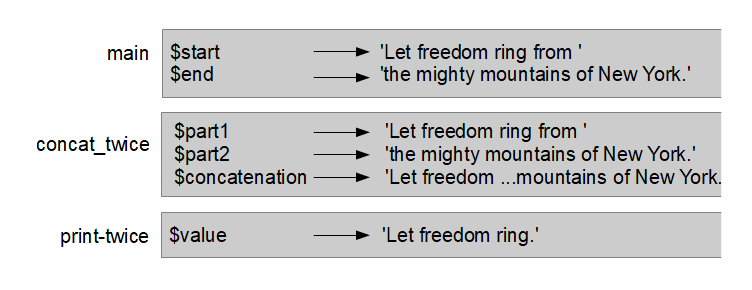
\includegraphics[scale=0.8]{figs/stack_diagram.png}}
%{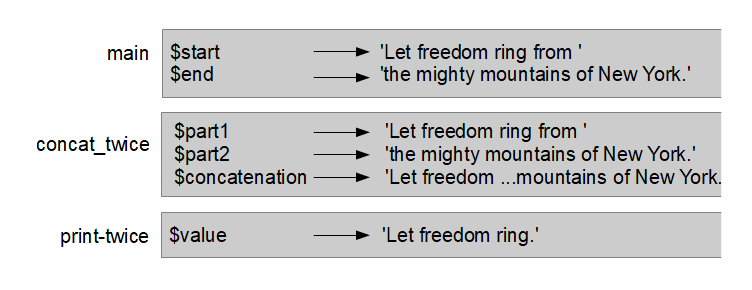
\includegraphics[scale=1.2]{figs/stack_diagram.png}}
\caption{Stack diagram.}
\label{fig.stack}
\end{figure}

Los marcos están organizados en la pila para indicar cual función
llama a cual. En este ejemplo, \verb|doble-impresión| fue llamada
por \verb|doble_concat|, y \verb|doble_concat| fue llamada por 
\verb|main|, el cual es un nombre especial para el marco superior.
Cuando creas una variable fuera de cualquier función, dicha variable
le pertenece a \verb|main|.

Cada parámetro hace referencia al mismo valor que su argumento correspondiente.
Así que, {\tt \$parte1} tiene el mismo valor que {\tt \$inicio},
{\tt \$parte2} tiene el mismo valor que {\tt \$final} y {\tt \$valor}
tiene el mismo valor que {\tt \$concatenación}.



\section{Fruitful Functions and Void Functions}
\index{fruitful function}
\index{void function}
\index{function, fruitful}
\index{function, void} 

Some of the functions we have used, such as the 
math functions, return results and are useful only insofar 
we use that return value; for lack of a better name, we 
may call them {\bf fruitful functions}.  Other functions, 
like \verb"print-twice", perform an action but don't appear 
to return a value (it does in fact return a value, {\tt True}, 
but we don't care about it).  They are sometimes called empty or 
{\bf void functions} in some other programming languages.

In some programming languages, such as Pascal or Ada, there 
is a strong distinction between a \emph{function} (which 
returns a value) and a \emph{procedure} (which doesn't); 
they are even defined with different keywords. This 
distinction does not apply to Perl and to most modern 
programming languages.

In fact, from a pure syntactic standpoint, Perl functions 
always return a result. So the distinction between 
``fruitful'' and ``void'' functions does not really exist 
syntactically, but only semantically, i.e., from the 
standpoint of the meaning of the program: maybe we need to 
use the return value, or maybe we don't.

Another distinction commonly made is between functions and 
mutators: functions do not change the initial state of the 
arguments they were called on, and mutators do modify it. We 
will not use this distinction here, but it is useful to 
keep it in mind.

When you call a fruitful function, you almost always
want to do something with the result; for example, you might
assign it to a variable or use it as part of an expression:

\begin{verbatim}
my $height = sin $radians;
my $golden = (sqrt(5) + 1) / 2;
\end{verbatim}
%
When you call a function in interactive mode (under the 
REPL), Perl usually displays the result:

\begin{verbatim}
> sqrt 5;
2.23606797749979
\end{verbatim}
%
But in a script, if you call a fruitful function all by 
itself, the return value is lost forever! In some cases, the 
compiler will be able to warn you, but not always. For example, 
consider the following program:

\begin{verbatim}
my $five = 5;
sqrt $five;
say $five;
\end{verbatim}

It produces the following warning:

\begin{verbatim}
WARNINGS for /home/Laurent/perl6_tests/sqrt.pl6:
Useless use of "sqrt $five" in expression "sqrt $five" in sink context (line 2)
5
\end{verbatim}
%
This script computes the square root of 5, but since 
it doesn't store or display the result, it is not very useful.
\index{interactive mode}
\index{script mode}

Void functions might display something on the screen, 
save some data to a file, modify a variable or an object, 
or have some other effect, but they generally don't have 
a return value, or at least not a useful one.  If you assign 
the result to a variable, you may get the return value of 
the subroutine, the value of the last expression which was 
evaluated in the function, or a special value such as 
{\tt Any}, which essentially means something that has not 
been defined, or {\tt Nil}.
\index{Any special value}
\index{special value!Any}
%

The subroutines we have written so far were essentially 
printing things to the screen. In that case, they 
usually return {\tt True}, at least when the printing 
was successful. Although they return a true value, what they 
return isn't very useful and we can consider them all void 
for our practical purposes.  

The following is an example of a very simple fruitful subroutine:
\index{return}

\begin{verbatim}
> sub square($number) { return $number ** 2 }
sub square ($number) { #`(Sub|118134416) ... }
> say square 5;
25
\end{verbatim}

The \verb'Sub|118134416' message displayed by the REPL is 
just an internal identifier for the subroutine we've just 
defined.

The {\tt return} statement instructs the function to terminate 
the execution of the function at this statement and to return 
the value of the following expression to the caller. In such a simple 
case where the program is in fact running the last statement 
of a function, the return keyword can be omitted since the function 
will return the value of the last evaluated statement, so that the 
{\tt square} subroutine could be written this way:
\begin{verbatim}
sub square($number) { 
    $number ** 2 
}
\end{verbatim}

We will be using fruitful functions more intensively in a 
few chapters.

\section{Function Signatures}
\index{function!signature}
\index{signature}

When a function receives arguments, which are stored into 
parameters, the part of the function 
definition describing the parameters between parentheses 
is called the {\bf function signature}. The function signatures 
we have seen so far are very simple and consist only of one 
parameter or possibly a parameter list.

Signatures can provide a lot more information about the 
parameters used by a function. First, you may define the 
type of the parameters. Some functions make sense only if their 
parameters are numeric and should probably raise an error if 
they get a string that cannot be converted to a numeric value. 
For example, if you define a function {\tt half} that computes 
a value equal to its argument divided by 2, it does not make 
sense to try to compute half of a string that is not numeric. 
It could be written as follows:
\index{type!parameter}
\index{parameter type}

\begin{verbatim}
sub half(Int $number) { 
    return $number / 2 
}
say half 84; # -> 42
\end{verbatim}

If this function is called with a string, we get the 
following error:
\index{type!String}

\begin{verbatim}
> say half "Douglas Adams"
===SORRY!=== Error while compiling <unknown file>
Calling half(Str) will never work with declared signature (Int $number)
at <unknown file>:1
------> say <HERE>half "Douglas Adams"
\end{verbatim}

The {\tt Int} type included in the function signature is a type 
constraint that can help prevent subtle bugs. In some cases, 
it can also be an annoyance. Consider this code snippet:
\index{constraint!type}
\index{type!constraint}
\index{type!Int}
\index{signature}


\begin{verbatim}
sub half(Int $number) {  $number / 2 }
say half "84"; # -> ERROR
\end{verbatim}

Because the argument to the {\tt half} subroutine is {\tt "84"}, 
i.e., a string, this code will fail with a type error. If we had 
not included the {\tt Int} type in the signature, the script 
would have converted (or \emph{coerced}) the "84" string to 
a number, divided it by two, and printed out the expected result:
\index{type!String}
\index{type!coercion}
\index{coercion!type}

\begin{verbatim}
sub half($number) { $number / 2 }
say half "84"; # -> 42
\end{verbatim}

In some cases, you want this conversion to occur, in others 
you don't. It is up to you to decide whether you want 
strict typing or not, depending on the specific situation and
needs. It is probably helpful to use parameter typing in many 
cases, but it can also become a straitjacket in some situations. 
Perl~6 lets you decide how strict you want to be about these things.

Our original {\tt half} subroutine has another limitation: it
can work only on integers. But a function halving its argument 
should presumably be useful for rational or even other numbers. 
You can use the {\tt Real} or {\tt Numeric} types to make 
the function more general (the difference between the two 
types is that the {\tt Numeric} type will accept not only 
{\tt Real} but also {\tt Complex} numbers\footnote{~Complex 
numbers are a powerful concept of mathematics. They are numbers 
of the form $a + bi$, where $a$ and $b$ are usual real number and 
$i$ an imaginary number such that $i^2$ equals $-1$.}). As it turns out 
that this {\tt half} function will also work correctly 
with complex numbers, choosing a {\tt Numeric} 
type opens more possibilities:
\index{Numeric type}
\index{type!Numeric}
\index{Real type}
\index{type!Real}
\index{Complex type}
\index{type!Complex}
\index{type!Int}

\begin{verbatim}
sub half(Numeric $number) { $number / 2 }
say half(3+4i); # -> 1.5+2i
\end{verbatim}

The following table sums up and illustrates some of the 
various types we have seen so far.

\begin{center}
\begin{tabular}{|l|c|}  \hline
\label{types}
\emph{Type} & \emph{Example}   \\ \hline
String      & \verb'"A string"', \verb"'Another string'", \verb'"42"' \\ \hline
Integer     & \verb' -3, -2, 0, 2, 42' \\ \hline
Rational    & \verb' 1/2, 0.5, 3,14159, 22/7, 42.0' \\ \hline
Real        & $\pi$, pi, $\surd{2}$, \emph{e}, $\log 42$, $\sin 0.7$\\ \hline
Complex     & $5.4 + 3i$ \\ \hline
\end{tabular}
\end{center}
\index{String type}
\index{type!String}


\section{Immutable and Mutable Parameters}

\index{immutable parameter}
\index{mutable parameter}
\index{parameter!mutable}
\index{parameter!immutable}
By default, subroutine parameters are {\bf immutable} aliases for 
the arguments passed to the subroutine. In other words, they 
cannot be changed within the function and you cannot 
accidentally modify the argument in the caller:

\begin{verbatim}
sub plus-three(Int $number) { $number += 3}
my $value = 5;
say plus-three $value; # ERROR: Cannot assign to an immutable value
\end{verbatim}

In some other languages, this behavior is named a ``call 
by value'' semantic: loosely speaking, the subroutine 
receives (by default) a value rather than a variable, and 
the parameter therefore cannot be modified.
\index{call by reference}

If you want to change the value of the parameter within the 
subroutine (but without changing the argument in the caller) 
you can add the {\tt is copy} \emph{trait} to the signature:
\index{signature}
\index{trait}
\index{is copy trait}
\index{trait!is copy}

\begin{verbatim}
sub plus-three(Int $number is copy) { $number += 3}
my $value = 5;
say plus-three $value;  # 8
say $value;             # 5 (unchanged)
\end{verbatim}
%
A {\bf trait} is a property of the parameter defined at compile time. 
Here, the {\tt \$number} parameter is modified within the 
subroutine and the incremented value is returned to the caller 
and printed as 8, but, within the caller, the variable used
as an argument to the function, {\tt \$value}, is not 
modified (it is still 5).

Although this can sometimes be dangerous, you may also want 
to write a subroutine that modifies its argument at the caller 
side. For this, you can use the {\tt is rw} \emph{trait} 
in the signature:
\index{is rw trait}
\index{trait!is rw}

\begin{verbatim}
sub plus-three(Int $number is rw) { $number += 3}
my $value = 5;
say plus-three $value;  # 8
say $value;             # 8 ($value modified)
\end{verbatim}
%
With the {\tt is rw} trait, the {\tt \$number} parameter is 
now  \emph{bound} to the {\tt \$value} argument, so that any change 
made using {\tt \$number} within the subroutine will immediately 
be applied to {\tt \$value} at the caller side, because {\tt \$number} 
and {\tt \$value} are just different names for the same thing (they 
both refer to the same memory location). The argument is now 
fully \emph{mutable}.

In some other languages, this is named a ``call by reference'' 
parameter passing mechanism, because, in those languages, if you 
pass to a function  a reference (or a pointer) to a variable, then 
it is possible for the function to modify the variable referred 
to by the reference.
\index{call by reference}


\section{Functions and Subroutines as First-Class Citizens}
\index{first-class object}
\index{object, first-class}
\index{function!higher-order}
\label{first_class}

Subroutines and other code objects can be passed around as values, 
just like any variable, literal, or object. Functions are said 
to be {\bf first-class objects} or sometimes first-class 
citizens or higher-order functions. This means that a Perl 
function (its code, not the value returned by it) is a value 
you can assign to a variable or pass around as an argument. 
For example, \verb"do-twice" is a subroutine that takes a 
function as an argument and calls it twice:

\begin{verbatim}
sub do-twice($code) {
    $code(); 
    $code();
}
\end{verbatim}

Here, the \verb"$code" parameter refers to a function or some
other callable code object. This is an example that uses
\verb"do-twice" to call a function named \verb"greet" twice:

\begin{verbatim}
sub greet {
    say "Hello World!";
}
do-twice &greet;
\end{verbatim}

This will print:
\begin{verbatim}
Hello World!
Hello World!
\end{verbatim}

The \verb"&" sigil placed before the subroutine name in the 
argument list tells Perl that you are passing around a 
subroutine or some other callable code object (and not 
calling the subroutine at the moment).
\index{sigil}
\index{ampersand sigil}
%\index{$&$ sigil}
%\index{sigil!$&$}

In fact, it would be more idiomatic to also use the \verb"&" 
sigil in the \verb"do-twice" subroutine definition, to better 
specify that the parameter is a callable code object:
\index{idiomatic}

\begin{verbatim}
sub do-twice(&code) {
    &code(); 
    &code();
}
\end{verbatim}

or even:
\begin{verbatim}
sub do-twice(&code) {
    code(); 
    code();
}
\end{verbatim}

The syntax with the \verb"&" sigil has the benefit that 
it will provide a better error message if you make a mistake 
and pass something noncallable to \verb"do-twice". 

All the functions we have seen so far had a name, but a 
function does not need to have a name and can be \emph{anonymous}. 
For example, it may be stored directly in a scalar variable:
\index{anonymous function}
\index{function!anonymous}

\begin{verbatim}
my $greet = sub {
    say "Hello World!";
};
$greet();               # prints "Hello World"
do-twice $greet;        # prints "Hello World" twice
\end{verbatim}

It could be argued that the above \verb"$greet" subroutine  
is not really anonymous, since it is stored into a scalar 
variable that could in a certain way be considered as its name. 
But the subroutine really has no name; it just happens to be 
assigned to a scalar variable. Just to show that the subroutine 
can really have no name at all, consider this:

\begin{verbatim}
do-twice(sub {say "Hello World!"} );
\end{verbatim}

It will happily print "Hello World" twice. If the \verb"$do-twice"
function was declared earlier, you can even simplify the syntax 
and omit the parentheses:

\begin{verbatim}
do-twice sub {say "Hello World!"};
\end{verbatim}

For such a simple case where there is no need to pass an 
argument or return a value, you can even omit the 
\verb"sub" keyword and pass a code block directly to the function:
\index{code block}

\begin{verbatim}
do-twice {say "Hello World!"};
do-twice {say "what's up doc"};
\end{verbatim}

As you can see, \verb"do-twice" is a \emph{generic} subroutine in 
charge of just performing twice any function or code 
block passed to it, without any knowledge about what 
this function or code block is doing. This is a powerful 
concept for some relatively advanced programming techniques 
that we will cover later in this book.
\index{generic subroutine}

Subroutines may also be passed as return values from other 
subroutines:
\index{factory, function}
\index{function!factory}

\begin{verbatim}
> sub create-func ($person) { return sub { say "Hello $person!"}}
# Creating two greeting functions
sub create-func ($person) { #`(Sub|176738440) ... }
> my $greet_world = create-func "World";
sub () { #`(Sub|176738592) ... }
> my $greet_friend = create-func "dear friend";
sub () { #`(Sub|176739048) ... }
# Using the greet functions
> $greet_world();
Hello World!
> $greet_friend();
Hello dear friend!
\end{verbatim} 

Here, \verb"create-func" returns a subroutine greeting someone. 
It is called twice with two different arguments in order to 
create two different functions at runtime, \verb"$greet_world" and 
\verb"$greet_friend". A function such as \verb"create-func" 
is sometimes a \emph{function factory} because you may create as many 
functions as you like by just calling \verb"create-func". This 
example may seem to be a slightly complicated way of doing 
something quite simple. At this point, it is 
just a bit too early to give really useful examples, but 
this is also a very powerful programming technique.  

We'll come back to these techniques in various places in this 
book and even devote an entire chapter (chapter~\ref{functional 
programming}) to this subject and related topics.


\section{Why Functions and Subroutines?}
\index{function, reasons for}

It may not be clear why it is worth the trouble to divide
a program into functions or subroutines.  There are 
several reasons:

\begin{itemize}

\item Creating a new subroutine gives you an opportunity to 
name a group of statements, which makes your program easier 
to read and debug. Subroutines also help making the flow of 
execution clearer to the reader.

\item Subroutines can make a program smaller by eliminating 
repetitive code.  Later, if you make a change, you only have
to make it in one place.
\index{code repetition}

\item Dividing a long program into subroutines allows you 
to debug the parts one at a time and then assemble them 
into a working whole.

\item Well-designed subroutines are often useful for many programs.
Once you write and debug one, you can reuse it.
\index{code reuse}

\index{abstraction}
\item Creating subroutines is one of the major ways to 
break up a difficult problem into smaller easier subtasks 
and to create successive layers of abstraction, which are 
the key to solve complex problems.
\index{abstraction}

\index{black box}
\item Writing good subroutines lets you create black boxes, with 
a known input and a known output. So you don't have to think 
about them anymore when you're working on something else.  
They've become a tool.  Once you've assembled an electric 
screwdriver, you don't need to think about how it works internally 
when you use it to build or repair something.
\index{black box}

\item In the current open source world, chances are that your 
code will have to be understood, maintained, or enhanced by 
people other than you. Coding has become much more of a social 
activity than before. Breaking up your code into small subroutines 
whose purpose is easy to understand will make their work easier. 
And you'll be even more delighted when the person 
having to maintain or refactor your code is... you.
\index{open source code}

\end{itemize}


\section{Debugging}

One of the most important programming skills you will 
acquire is debugging. Although it can sometimes be 
frustrating, debugging is one of the most intellectually 
rich, challenging, and interesting parts of programming.
\index{experimental debugging}
\index{debugging!experimental}

In some ways debugging is like detective work.  You are confronted
with clues and you have to infer the processes and events that led
to the results you see.

Debugging is also like an experimental science.  Once you have an idea
about what is going wrong, you modify your program and try again.  If
your hypothesis was correct, you can predict the result of the
modification, and you take a step closer to a working program.  If
your hypothesis was wrong, you have to come up with a new one.  As
Sherlock Holmes pointed out, ``When you have eliminated the
impossible, whatever remains, however improbable, must be the truth''
(A. Conan Doyle, {\em The Sign of Four}).
\index{Holmes, Sherlock}
\index{Conan Doyle, Arthur}

In cases where you are not able to come up with a hypothesis 
on what's wrong, you can try to introduce code that you expect 
to create a certain type of error, a ``negative hypothesis'' 
if you will.  Sometimes you can learn a lot from the fact that 
it didn't create the error that was expected. Making a hypothesis 
does not necessarily mean you have an idea about how to make it 
work, it could also be a hypothesis on how it should break.

For some people, programming and debugging are the same thing.  That
is, programming is the process of gradually debugging a program until
it does what you want.  The idea is that you should start with a
working program and make small modifications,
debugging them as you go.

For example, Linux is an operating system that contains millions of
lines of code, but it started out as a simple program Linus Torvalds
used to explore the Intel 80386 chip.  According to Larry Greenfield,
``One of Linus's earlier projects was a program that would switch
between printing \verb"AAAA" and \verb"BBBB".  This later evolved 
to Linux.'' ({\em The Linux Users' Guide} Beta Version 1).
\index{Linux}


\section{Glossary}

\begin{description}

\item[Function] A named sequence of statements that performs 
some useful operation. Functions may or may not take arguments 
and may or may not produce a result. Perl comes with many 
built-in functions, and you can also create your own. In Perl, 
user-defined functions are often called subroutines.
\index{function}

\item[Function definition]  A statement that creates a new function,
specifying its name, parameters, and the statements it contains.
\index{function!definition}

\item[Header] The first line of a function definition.
\index{header}

\item[Body] The sequence of statements inside a function 
definition, usually in a code block delimited by braces.
\index{body}

\item[Parameter] A name used inside a subroutine to refer to 
the value passed as an argument.
\index{parameter}

\item[Function call] A statement that runs a function. It
consists of the function name followed by an argument list, 
which may or may not be enclosed within parentheses.
\index{function!call}

\item[Argument]  A value provided to a function when the function is called.
This value is assigned to the corresponding parameter in the function.
\index{argument}

\item[Lexical variable]  A variable defined inside a subroutine 
or a code block.  A lexical variable defined within a function can 
only be used inside that function.
\index{local variable}

\item[Return value]  The result of a function.  If a function call
is used as an expression, the return value is the value of
the expression.
\index{return!value}

\item[Any]  A special value typically found in variables that 
haven't been assigned a value. It is also a special value 
returned by some functions that we have called ``void'' (because 
they return something generally useless such as ``Any'').
\index{Any special value}
\index{special value!Any}

\item[Nil] Also a special value sometimes returned by some 
``void'' subroutines.

\item[Module] A file that contains a
collection of related functions and other definitions.
\index{module}

\item[Use statement] A statement that reads a module file and usually imports some functions.
\index{use statement}
\index{statement!use}

\item[Composition] Using an expression as part of a larger expression,
or a statement as part of a larger statement.
\index{composition}

\item[Flow of execution]  The order in which statements run.
\index{flow of execution}

\item[Stack diagram]  A graphical representation of a stack of subroutines,
their variables, and the values they refer to.
\index{stack diagram}

\item[Frame]  A box in a stack diagram that represents a subroutine call.
It contains the local variables and parameters of the subroutine.
\index{function!frame}
\index{frame}

\item[Fruitful function] A function or subroutine that returns a useful value.
\index{fruitful function}

\item[Void function] A function or subroutine that does not 
return a useful value.
\index{void function}

\item[Function signature] The part of the definition of a 
function (usually between parentheses) that defines its 
parameters and possibly their types and other properties.
\index{function!signature}
\index{signature}

\item[Immutable parameter] A function or subroutine parameter 
that cannot be changed within the function body. By default, 
subroutine parameters are immutable.
\index{immutable parameter}

\item[Trait] A property of a function or subroutine parameter 
that is defined at compile time.
\index{trait}

\item[First class object] Perl's subroutines are said to be
higher order objects or first-class objects, because they can 
be passed around as other subroutines' arguments or return values, 
just as any other objects.
\index{first-class object}
\index{object, first-class}

\item[Anonymous function] A function that has no name.
\index{anonymous function}
\index{function!anonymous}

\item[Function factory] A function that produces other functions as return values.
\index{factory, function}
\index{function!factory}

\end{description}


\section{Exercises}

\begin{exercise}
\index{chars function}
\index{function!chars}
\label{right_justify}

Write a subroutine named \verb"right-justify" that takes a string
named {\tt \$input-string} as a parameter and prints the 
string with enough leading spaces so that the last letter 
of the string is in column 70 of the display.

\begin{verbatim}[fontshape=up]
> right-justify('Larry Wall')
                                                           Larry Wall
\end{verbatim}

Hint: use string concatenation and repetition.  Also,
Perl provides a built-in function called {\tt chars} that
returns the length of a string, so the value of 
\verb"chars 'Larry Wall'" or \verb"'Larry Wall'.chars" is 10.
Solution: \ref{sol_right_justify}.

\end{exercise}


\begin{exercise}
\index{first-class object}
\index{object!first-class}
\index{do-twice}
\label{do_it_twice}


We have seen that functions and other code objects can be 
passed around as values, just like any object. Functions are said 
to be \emph{first-class objects}. For example, \verb"do-twice" is a function
that takes a function as an argument and calls it twice:

\begin{verbatim}[fontshape=up]
sub do-twice($code) {
    $code(); 
    $code();
}
sub greet {
    say "Hello World!";
}
do-twice(&greet);
\end{verbatim}

\begin{enumerate}

\item Type this example into a script and test it.

\item Modify \verb"do-twice" so that it takes two arguments, a
function and a value, and calls the function twice,
passing the value as an argument.

\item Copy the definition of 
\verb"print-twice" from earlier in this chapter to your script.

\item Use the modified version of \verb"do-twice" to call
\verb"print-twice" twice, passing ``What's up doc'' as an argument.

\item Define a new function called 
\verb"do-four" that takes a function and a value
and calls the function four times, passing the value
as a parameter.  There should be only
two statements in the body of this function, not four.

\end{enumerate}

Solution: \ref{sol_do_it_twice}.

\end{exercise}



\begin{exercise}
\label{draw_a_grid}
\index{print-grid}

Note: This exercise should be
done using only the statements and other features we 
have learned so far.  

\begin{enumerate}

\item Write a subroutine that draws a grid like the following:
\index{grid}

\begin{verbatim}[fontshape=up]
+ - - - - + - - - - +
|         |         |
|         |         |
|         |         |
|         |         |
+ - - - - + - - - - +
|         |         |
|         |         |
|         |         |
|         |         |
+ - - - - + - - - - +
\end{verbatim}
%
Hint: to print more than one value on a line, you can print
a comma-separated sequence of values:

\begin{verbatim}[fontshape=up]
  say '+', '-';
\end{verbatim}
%
The {\tt say} function prints its arguments with a newline at the end (it advances to the next line). If you don't want to 
go to the next line, use the {\tt print} function instead:


\begin{verbatim}[fontshape=up]
  print '+', ' ';
  print '-';
\end{verbatim}
%
The output of these statements is ``+ -''.

A {\tt say} statement with an empty string argument ends 
the current line and goes to the next line.

\item Write a subroutine that draws a similar grid
with four rows and four columns.

\end{enumerate}

Solution: \ref{sol_draw_a_grid}
\index{print-grid}.

Credit: this exercise is based on an exercise in Oualline, {\em
    Practical C Programming, Third Edition}, O'Reilly Media, 1997.

\end{exercise}

